\section{Esperienza \S~38}

L'esperienza del \S~38, descritta nel capitolo V del volume di Righi~\cite{righi1897ottica} (pagina 148 del libro), 
ha per oggetto la riflessione delle onde elettromagnetiche. Prima di descriverla è però opportuno richiamare il 
concetto di riflessione (fig \ref{fig:riflessione_theta}) e la legge che la governa.\\
Tale legge afferma che l'angolo di incidenza di un raggio luminoso è uguale all'angolo di riflessione:
\begin{equation}
    \theta_i = \theta_r .
    \label{eq:legge-riflessione}
\end{equation}

La sua formulazione più antica è tradizionalmente attribuita a Euclide (circa 300~a.C.), nel trattato di Ottica.\\ 
La legge di riflessione come la conosciamo oggi è:

\begin{figure}[htbp]
    \centering
    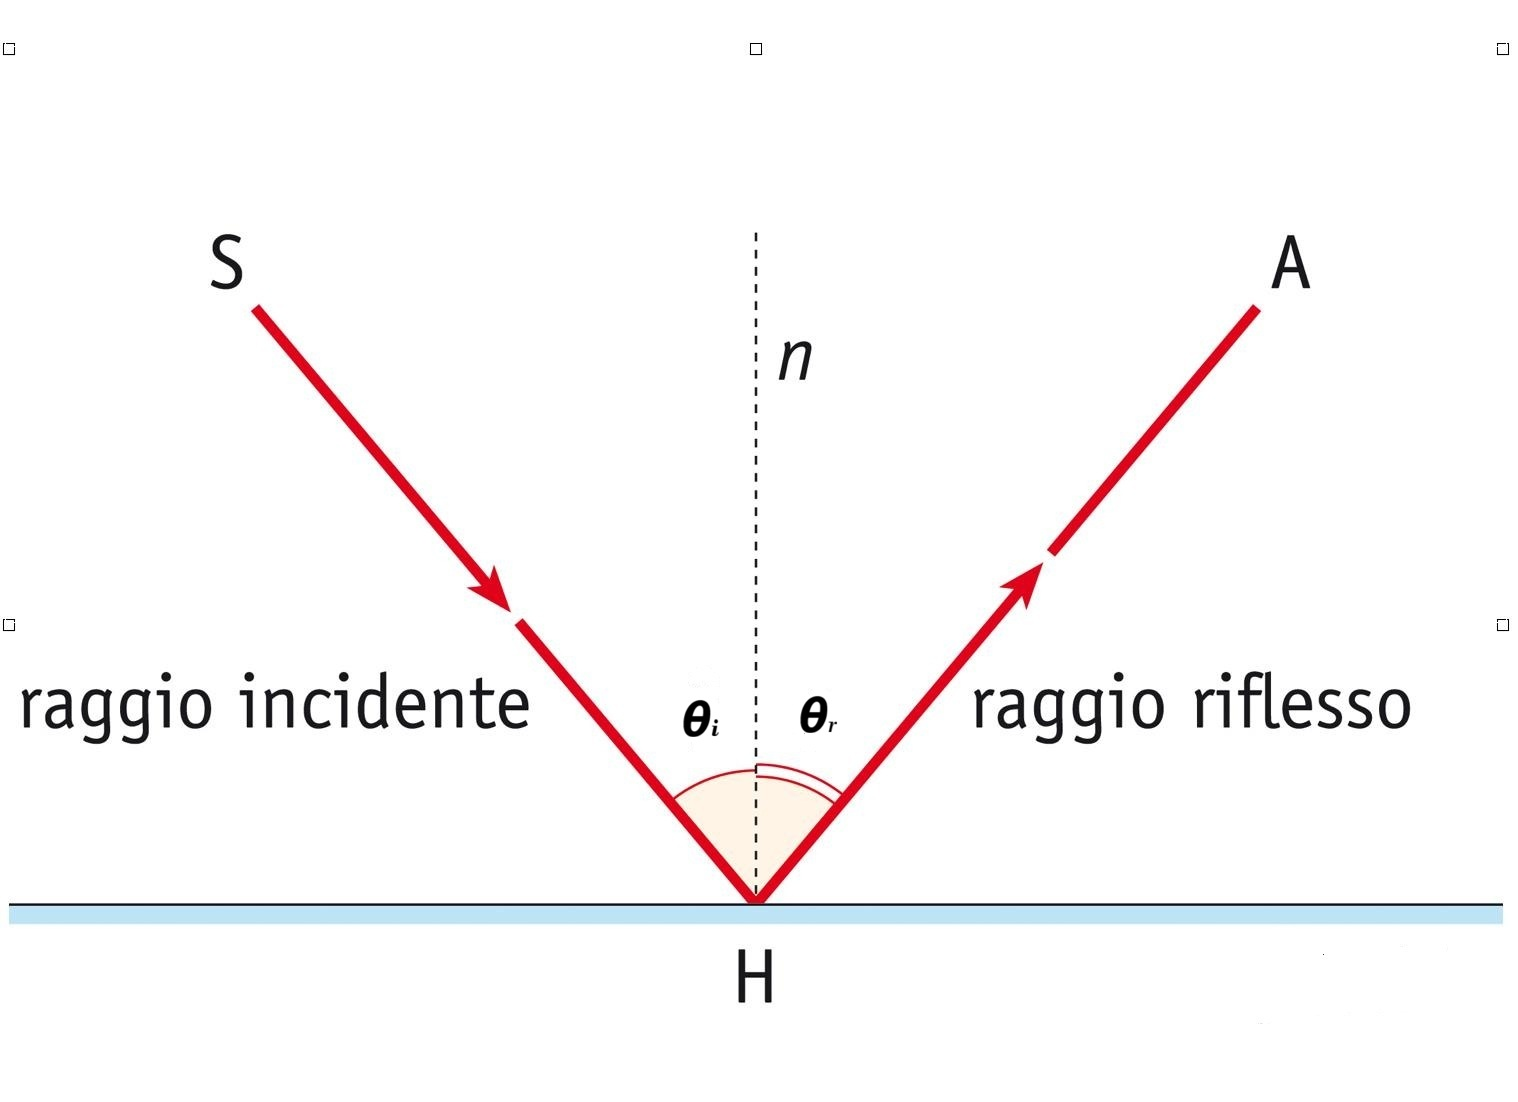
\includegraphics[width = 0.8\textwidth]{immagini/riflessione_theta.jpg}
    \caption{Schema della legge di riflessione}
    \label{fig:riflessione_theta}
\end{figure}

\subsection{Set up sperimentale}

La descrizione dell'esperimento inizia con "specchi sferici concavi di metallo" di 44 cm di diametro e 18.6 cm di distanza focale ($f$),
inizialmente "\textit{adoperati nelle lezioni per la riflessione del suono e del calore}". \\
Ragionando in 2-D (fig \ref{fig:specchio_concavo}) e usando la trigonometria risulta che:
\begin{itemize}
    \item il raggio di curvatura ($R$) dello specchio è $R = 2f = 37.2$ cm, 
    \item il semiangolo di apertura dello specchio è $\alpha = \arcsin{\frac{D/2}{R}} \approx 36^\circ$.
\end{itemize}

\begin{figure}[htbp]
    \centering
    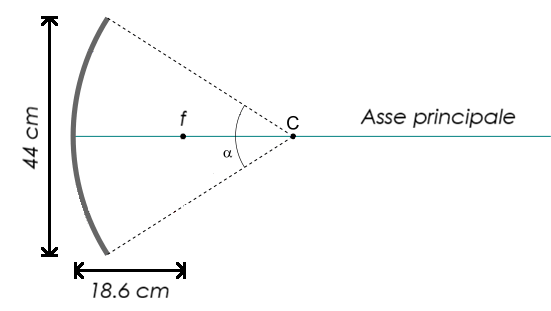
\includegraphics[width = 0.8\textwidth]{immagini/schema_specchio_concavo.png}
    \caption{Schema dello specchio concavo}
    \label{fig:specchio_concavo}
\end{figure}

Tornando all'esperienza di Righi, l'apparato sperimentale da lui impiegato per la verifica della legge di riflessione è il seguente:

\begin{itemize}
    \item \textbf{Emettitore/Oscillatore ($O$)}: un oscillatore a quattro sfere con le due centrali immerse in olio di vaselina (ideato dal fisico bolognese stesso), posizionato lungo la linea focale di uno specchio cilindrico parabolico di rame ($M_1$). Tale riflettore concentra l'energia emessa proiettando uno stretto fascio di radiazioni parallele e linearmente polarizzate.
    \item \textbf{Superficie riflettente ($S$)}: un'ampia lastra piana (metallica o di materiale dielettrico come vetro o paraffina) disposta verticalmente al centro di una piattaforma goniometrica graduata ($P$). La lastra può essere ruotata per impostare con precisione l'angolo di incidenza $\theta_i$ rispetto alla normale $N$ alla superficie.
    \item \textbf{Rilevatore/Risonatore ($R$)}: un risonatore a striscia d'argento interrotta, posto nel fuoco di un secondo specchio cilindrico parabolico ($M_2$). Questo secondo specchio è montato su un braccio metallico orientabile che ruota attorno all'asse centrale del goniometro $P$, consentendo di misurare l'intensità del segnale riflesso a qualsiasi angolo $\theta_r$.
\end{itemize}

\begin{figure}[htbp]
    \centering
    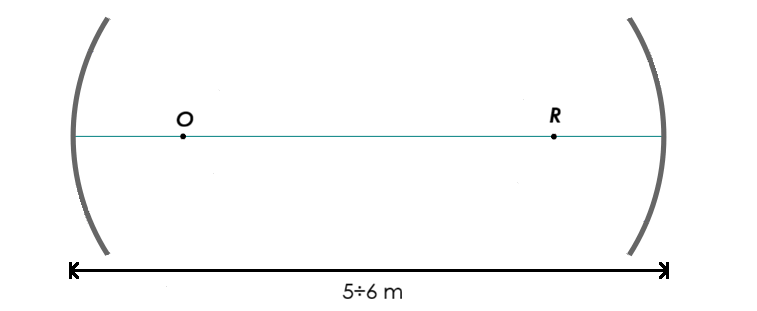
\includegraphics[width = 0.8\textwidth]{immagini/schema_esp_base.png}
    \caption{Schema dell'apparato sperimentale: O è l'oscillatore, R è il risonatore.}
    \label{fig:setup-base}
\end{figure}

% \begin{figure}[htbp]
%     \centering
%     \includegraphics[width = 0.85\textwidth]{immagini/setup_esperimento_38.png}
%     \caption{Schema dell'apparato sperimentale adoperato da Righi per la verifica delle leggi della riflessione ($\theta_i = \theta_r$).}
%     \label{fig:setup-riflessione}
% \end{figure}

Durante l'esecuzione dell'esperienza, inviando il fascio incidente con un angolo $\theta_i$ prefissato e facendolo incidere sulla lastra $S$, Righi ruota il braccio del risonatore $R$ registrando la brillantezza delle scintille. La massima luminosità della scarica si osserva con rigorosa precisione \textbf{esclusivamente quando l'angolo di riflessione coincide con l'angolo di incidenza} ($\theta_r = \theta_i$). Inoltre, spostando il risonatore al di sopra o al di sotto del piano d'incidenza orizzontale, le scintille cessano immediatamente, confermando sperimentalmente che il raggio riflesso giace nello stesso piano individuato dal raggio incidente e dalla normale alla superficie \cite{righi1897ottica}.

\paragraph{Analogia con la conduzione in tubo metallico.}
A completamento del \S~38, Righi descrive un'ulteriore ed elegante esperienza in cui colloca l'oscillatore all'estremità di un lungo tubo metallico cavo (simile a un comune tubo da stufa) e il risonatore all'estremità opposta. Le pareti metalliche interne fungono da specchio continuo, guidando l'onda elettromagnetica per successive riflessioni speculari interne senza dispersione spaziale (primo esempio di \emph{guida d'onda}). L'interruzione della radiazione mediante un disco conduttore interno ne conferma la natura di riflessione confinata, in perfetta analogia con la propagazione del suono nei tubi acustici o della luce in condotti a specchio \cite{righi1897ottica}.

\subsection{Considerazioni fisiche e implicazioni teoriche}

Dopo aver verificato le leggi puramente geometriche dell'ottica, Righi compie un fondamentale passaggio concettuale: dallo studio \emph{geometrico} della traiettoria dei raggi passa allo studio \emph{fisico} della natura vettoriale delle oscillazioni riflesse, analizzandone l'intensità, lo stato di fase e l'orientazione nello spazio \cite{righi1897ottica}.

\subsection{Naturale polarizzazione e prova della teoria di Maxwell}
Mentre la luce naturale visibile è emessa con piani di vibrazione casuali e disordinati, le onde elettromagnetiche generate dagli oscillatori a scarica nascono \textbf{intrinsecamente e totalmente polarizzate} rettilinealmente, con la direzione del campo elettrico definita dall'asse dell'oscillatore \cite{righi1897ottica}.

Questa proprietà permette a Righi di impostare un test cruciale per confrontare la teoria ottica ondulatoria classica di Fresnel con la teoria elettromagnetica di Maxwell \cite{righi1897ottica}:
\begin{itemize}
    \item Nella teoria elastica di Fresnel, la vibrazione dell'etere avvenga in direzione \emph{perpendicolare} al piano di polarizzazione.
    \item Nella teoria di Maxwell, il campo elettromagnetico è costituito da due vettori ortogonali: la forza elettrica ($\mathbf{E}$) e la forza magnetica ($\mathbf{H}$).
\end{itemize}
Righi dimostra sperimentalmente che la \textbf{forza elettrica corrisponde esattamente alla vibrazione dell'etere della teoria di Fresnel} (risultando perpendicolare al piano di polarizzazione), mentre la \textbf{forza magnetica giace nel piano di polarizzazione} \cite{righi1897ottica}. Questo risultato fornisce una conferma sperimentale diretta dell'identità tra vibrazioni luminose e oscillazioni elettromagnetiche \cite{righi1897ottica, righi1897ottica}.

\subsection{Fondamento per i fenomeni complessi della riflessione}
La verifica condotta nel \S~38 costituisce il presupposto metodologico per le indagini svolte nei paragrafi successivi del Capitolo V \cite{righi1897ottica}:
\begin{enumerate}
    \item \textbf{Riflessione sui dielettrici (\S~39--40)}: studio della variazione d'intensità dell'onda riflessa al variare dell'angolo d'incidenza su isolanti (vetro, paraffina, zolfo) e verifica dell'estinzione dell'onda all'\emph{angolo di Brewster}, confermando le formule di Fresnel.
    \item \textbf{Riflessione metallica ed ellittica (\S~41--43)}: analisi dello sfasamento introdotto dalla riflessione sui conduttori metallici (rame), che trasforma un'onda a polarizzazione rettilinea in un'onda a \emph{polarizzazione ellittica o circolare}.
\end{enumerate}

Attraverso queste esperienze, Righi dimostra che la riflessione delle onde radio segue in tutto e per tutto le medesime leggi e relazioni quantitative stabilite da Fresnel e Malus per la luce visibile, consolidando la sintesi elettromagnetica di Maxwell \cite{righi1897ottica}.

